% ==============================================================================
% หน้าปกตำราวิชาการ 3D Pixar Semi-realistics & Dual-Layer Drop-Shadow Typography
% Architecture: /academic-book-cover-architect
% ผู้ช่วยศาสตราจารย์ ดร.ชีวะ ทัศนา (ผู้ออกแบบและพัฒนา)
% ==============================================================================
\begin{titlepage}
\thispagestyle{empty}
\newgeometry{left=0mm, right=0mm, top=0mm, bottom=0mm}
\begingroup
\coverfont
\setlength{\XeTeXlinebreakskip}{0pt}
\begin{tikzpicture}[remember picture, overlay]

  % 1. Full-Bleed 100% 3D Pixar Semi-Realistic Artwork
  \node[anchor=center, inner sep=0pt] at (current page.center) {
      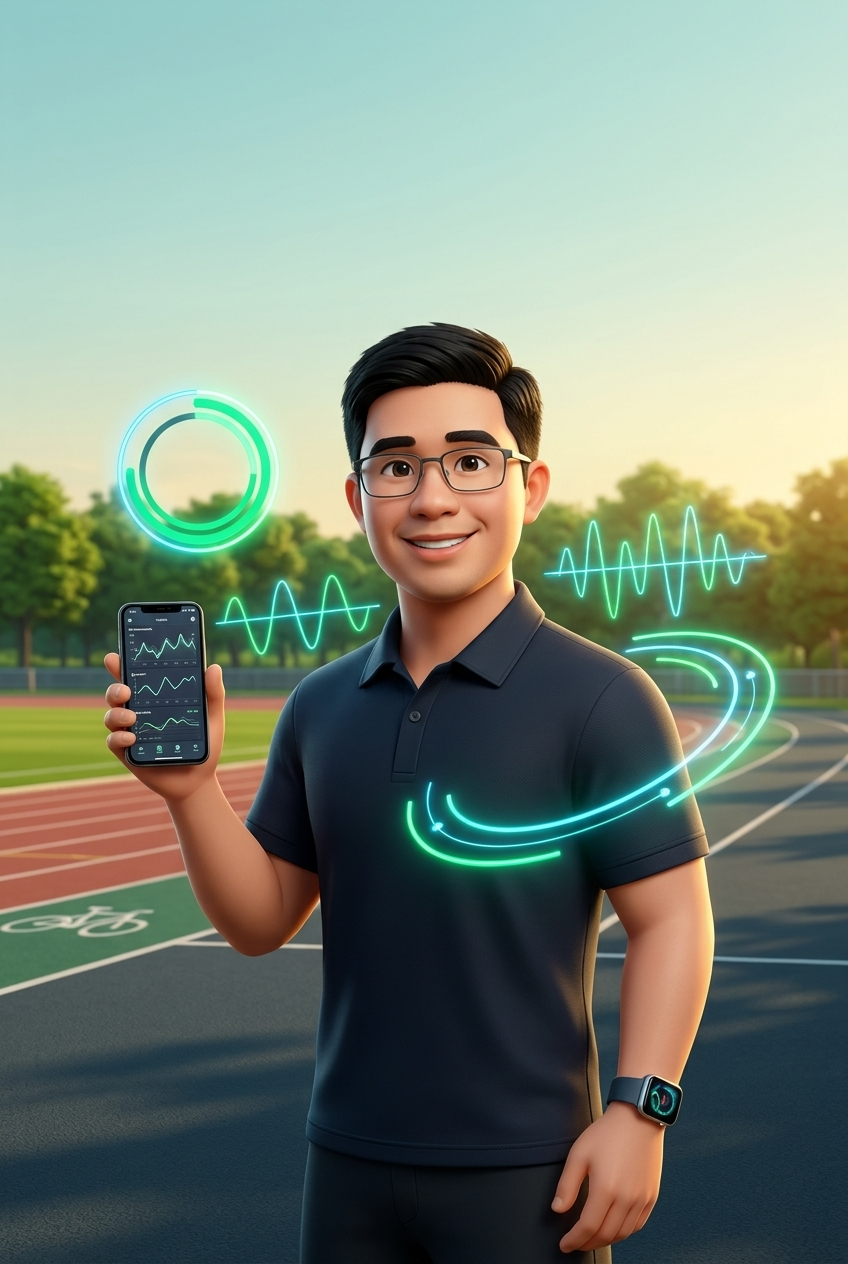
\includegraphics[width=\paperwidth,height=\paperheight]{figures/cover_art.jpg}
  };

  % ----------------------------------------------------------------------------
  % ZONE 1: UPPER 35% (NEGATIVE SPACE & DUAL-LAYER DROP-SHADOW TITLES)
  % ----------------------------------------------------------------------------
  % 1.1 Series Badge (Dual-Layer White Glow + Deep Teal)
  \node[anchor=north, align=center] at ([xshift=0.6pt, yshift=-11.4mm]current page.north) {
      {\fontsize{10.5}{14}\selectfont\bfseries\color{white} DIGITAL HEALTH \& BIOMECHANICS SERIES 2026 \textbullet\ มรภ.รำไพพรรณี}
  };
  \node[anchor=north, align=center] at ([xshift=-0.6pt, yshift=-12.6mm]current page.north) {
      {\fontsize{10.5}{14}\selectfont\bfseries\color{white} DIGITAL HEALTH \& BIOMECHANICS SERIES 2026 \textbullet\ มรภ.รำไพพรรณี}
  };
  \node[anchor=north, align=center] at ([yshift=-12.0mm]current page.north) {
      {\fontsize{10.5}{14}\selectfont\bfseries\color{rbruCyan!85!black} DIGITAL HEALTH \& BIOMECHANICS SERIES 2026 \textbullet\ มรภ.รำไพพรรณี}
  };

  % 1.2 Thai Title (Cluster-Safe Multicolor + Dual-Layer White Glow Shadow)
  \foreach \dx/\dy in {-1.2/0, 1.2/0, 0/-1.2, 0/1.2, -0.9/-0.9, 0.9/-0.9, -0.9/0.9, 0.9/0.9} {
    \node[anchor=north, align=center] at ([xshift=\dx pt, yshift=-21.0mm+\dy pt]current page.north) {
        {\fontsize{28}{34}\selectfont\bfseries\color{white} สมาร์ทเฮลท์แทร็กเกอร์และชีวกลศาสตร์}
    };
  }
  \node[anchor=north, align=center] at ([yshift=-21.0mm]current page.north) {
      {\fontsize{28}{34}\selectfont\bfseries%
       {\color{rbruBlue!90!black}สมาร์ท}%
       {\color{rbruEmerald!85!black}เฮลท์}%
       {\color{rbruCyan!90!black}แทร็กเกอร์}%
       {\color{rbruOrange!90!black}และชีวกลศาสตร์}}
  };

  % 1.3 Prominent English Title (Large Bold All-Caps + White Glow Shadow)
  \foreach \dx/\dy in {-1.0/0, 1.0/0, 0/-1.0, 0/1.0, 0.8/-0.8} {
    \node[anchor=north, align=center] at ([xshift=\dx pt, yshift=-36.5mm+\dy pt]current page.north) {
        {\fontsize{17.5}{22}\selectfont\bfseries\color{white} SMART HEALTH TRACKER \& KINEMATICS}
    };
  }
  \node[anchor=north, align=center] at ([yshift=-36.5mm]current page.north) {
      {\fontsize{17.5}{22}\selectfont\bfseries\color{rbruNavy} SMART HEALTH TRACKER \& KINEMATICS}
  };

  % 1.4 Subtitle (Dual-Layer White Glow + Slate Navy)
  \node[anchor=north, align=center] at ([xshift=0.6pt, yshift=-46.6mm]current page.north) {
      {\fontsize{10}{13.5}\selectfont\bfseries\color{white} ระบบนับก้าวไฮบริด \textbullet\ วิ่งและปั่นจักรยาน \textbullet\ พิกัดดาวเทียม GPS \textbullet\ ปัญญาประดิษฐ์เชิงลึก}
  };
  \node[anchor=north, align=center] at ([yshift=-46.0mm]current page.north) {
      {\fontsize{10}{13.5}\selectfont\bfseries\color{rbruSlate!95!black} ระบบนับก้าวไฮบริด \textbullet\ วิ่งและปั่นจักรยาน \textbullet\ พิกัดดาวเทียม GPS \textbullet\ ปัญญาประดิษฐ์เชิงลึก}
  };

  % ----------------------------------------------------------------------------
  % ZONE 3: BOTTOM 20% (DARK METADATA CANVAS & AUTHOR BLOCK)
  % ----------------------------------------------------------------------------
  % Deep Black Multi-Offset Drop-Shadow Layer
  \foreach \dx/\dy in {-1.2/0, 1.2/0, 0/-1.2, 0/1.2, 1.4/-1.4, -1.0/-1.0, 1.0/1.0, -1.0/1.0} {
    \node[anchor=south, align=center] at ([xshift=\dx pt, yshift=12.0mm+\dy pt]current page.south) {
        {\fontsize{17.5}{22.5}\selectfont\bfseries\color{black} ผู้ช่วยศาสตราจารย์ ดร.ชีวะ ทัศนา}\\[3.5pt]
        {\fontsize{11.5}{15}\selectfont\bfseries\color{black} ผู้ออกแบบและพัฒนา \textbullet\ สาขาวิชาฟิสิกส์ คณะวิทยาศาสตร์และเทคโนโลยี}\\[3pt]
        {\fontsize{10.5}{14}\selectfont\bfseries\color{black} มหาวิทยาลัยราชภัฏรำไพพรรณี \textbullet\ พ.ศ. ๒๕๖๙}
    };
  }

  % Foreground Crisp Author Layer
  \node[anchor=south, align=center] at ([yshift=12.0mm]current page.south) {
      {\fontsize{17.5}{22.5}\selectfont\bfseries\color{white} ผู้ช่วยศาสตราจารย์ ดร.ชีวะ ทัศนา}\\[3.5pt]
      {\fontsize{11.5}{15}\selectfont\bfseries\color{white!95} ผู้ออกแบบและพัฒนา \textbullet\ สาขาวิชาฟิสิกส์ คณะวิทยาศาสตร์และเทคโนโลยี}\\[3pt]
      {\fontsize{10.5}{14}\selectfont\bfseries\color{yellow!90!orange} มหาวิทยาลัยราชภัฏรำไพพรรณี \textbullet\ พ.ศ. ๒๕๖๙}
  };

\end{tikzpicture}
\endgroup
\restoregeometry
\end{titlepage}
\pagecolor{white}
